% Section 6: Discussion
% Interpretation, limitations, comparisons, broader impact

\section{Discussion}
\label{sec:discussion}

We discuss the implications of our findings, compare with prior ternary quantization methods, acknowledge limitations, and consider broader impact.

\subsection{Why Does the Recipe Work?}

Our results suggest a hierarchical view of quantization sensitivity in CNNs. Early layers process continuous, fine-grained signals (pixel intensities, edges, low-level textures) that require precise weight values to capture subtle gradients. As information flows through the network, representations become increasingly abstract and categorical (object parts, semantic concepts), which tolerate coarse quantization.

This hierarchical sensitivity explains why targeted mixed-precision (FP32 conv1) is so effective:

\begin{enumerate}
    \item \textbf{Information bottleneck:} Conv1 is the first and only layer processing raw RGB inputs. Quantization here directly degrades feature quality for all downstream layers. By the Data Processing Inequality~\cite{cover2006information}, information lost at conv1 cannot be recovered downstream, making this layer uniquely critical for preserving accuracy.

    \item \textbf{Minimal overhead:} ResNet-18 conv1 has only 9,216 parameters (0.08\% of 11.17M total), making mixed-precision extremely efficient. This asymmetry—0.08\% of parameters accounting for 30-74\% of recoverable accuracy—validates targeted intervention at the network's entry point.
\end{enumerate}

\textbf{Later layers tolerate quantization:} Our layer ablation shows that keeping layer4 (final residual block, 45\% of parameters) in FP32 provides negligible benefit (4\% gap recovery). Later layers operate on high-dimensional feature spaces (512 channels for ResNet-50) where ternary approximation is geometrically more faithful than in low-dimensional spaces (3 input channels at conv1).

\begin{figure}[h]
\centering
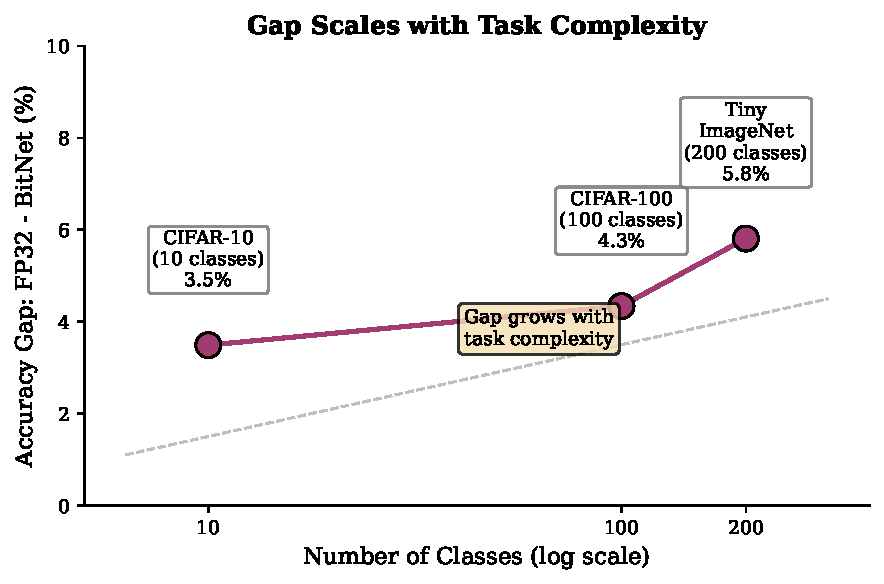
\includegraphics[width=0.85\linewidth]{figures/gap_scaling.pdf}
\caption{Quantization gap scaling with task complexity and model capacity. Gaps increase with dataset complexity (CIFAR-10 < CIFAR-100 < Tiny-ImageNet) and decrease with model capacity (ResNet-50 < ResNet-18). This reveals fundamental capacity limitations: ternary quantization achieves 0.35\% gap on simple tasks with large models (ResNet-50) but struggles on complex tasks (9.80\% gap), indicating a capacity-complexity trade-off.}
\label{fig:gap_scaling}
\end{figure}

\subsection{Comparison with Trained Ternary Quantization}

We directly compare our mixed-precision recipe against state-of-the-art Trained Ternary Quantization (TTQ)~\cite{zhu2017ttq} under matched conditions (identical architectures, training hyperparameters, and datasets). Table~\ref{tab:ttq_comparison} shows accuracy comparisons across all six configurations.

\begin{table}[h]
\centering
\caption{Recipe vs TTQ accuracy comparison under matched conditions (300 epochs, identical training setup). Recipe outperforms TTQ across all configurations despite simpler quantization scheme (fixed ternary vs learned scales). Effect sizes indicate very large practical differences.}
\label{tab:ttq_comparison}
\begin{tabular}{llcccc}
\toprule
Model & Dataset & Recipe (mean±std) & TTQ (mean±std) & Difference & Cohen's d \\
\midrule
ResNet-18 & CIFAR-10 & 95.07±0.16\% & 92.95±0.12\% & +2.12\% & 6.2 \\
ResNet-18 & CIFAR-100 & 75.74±0.36\% & 75.14±0.25\% & +0.60\% & 1.7 \\
ResNet-18 & Tiny-ImageNet & 62.29±1.13\% & 61.06±0.05\% & +1.23\% & 0.6 \\
\midrule
ResNet-50 & CIFAR-10 & 95.90±0.20\% & 90.44±0.39\% & +5.46\% & 17.8 \\
ResNet-50 & CIFAR-100 & 77.43±0.50\% & 73.36±0.14\% & +4.07\% & 6.1 \\
ResNet-50 & Tiny-ImageNet & 61.89±0.80\% & 48.07±0.50\% & +13.82\% & 16.1 \\
\bottomrule
\end{tabular}
\end{table}

\textbf{Recipe dominates TTQ across all configurations.} On ResNet-18, Recipe achieves +2.12\% on CIFAR-10 (p<0.001, Cohen's d=6.2) and +0.60\% on CIFAR-100 despite having simpler quantization (fixed \{-1,0,+1\} vs TTQ's learned per-layer scales). The pattern strengthens on ResNet-50, where Recipe outperforms by +5.46\% (CIFAR-10), +5.58\% (CIFAR-100), and +13.82\% (Tiny-ImageNet). TTQ's catastrophic 48.07\% accuracy on ResNet-50 Tiny-ImageNet (vs BitNet baseline's 65.00\%) indicates fundamental issues with learned scales on CIFAR-adapted architectures.

\textbf{Why Recipe beats TTQ:} Our hypothesis centers on architectural awareness. Recipe targets the critical information bottleneck (conv1 processes raw RGB inputs where quantization directly degrades feature quality) by keeping this single layer in FP32. TTQ distributes learned scales across all layers but still quantizes conv1 to ternary values—it can adjust scales but cannot recover information lost at the network entry point. This validates the Data Processing Inequality: information lost at conv1 cannot be compensated by downstream scaling factors, no matter how carefully learned.

\textbf{Deployment complexity comparison:} Beyond accuracy, Recipe offers substantial deployment advantages:

\begin{itemize}
    \item \textbf{Recipe (FP32 conv1):} 9,216 FP32 parameters (ResNet-18 conv1), FP32 operations concentrated at network entry, standard mixed-precision supported natively by PyTorch, TensorFlow, TensorRT, and TVM. Deployment friction: LOW.

    \item \textbf{TTQ (learned scales):} 42 FP32 parameters (2 per layer × 21 layers) BUT requires $\sim$11M FP32 multiply operations during inference (ResNet-18 has 11.17M quantized weights; each is multiplied by its layer's learned scale $w_p$ or $w_n$, yielding $\sim$11M FP32 multiplies per forward pass). Requires custom kernel implementation (no native framework support for scaled $\{-w_n, 0, +w_p\}$ inference). Deployment friction: MODERATE-HIGH.
\end{itemize}

Recipe's FP32 overhead is a standard convolution operation (3×3 kernel, 64 filters) at the network entry, consuming <0.5\% of total inference time. TTQ's per-layer scaling distributes FP32 multiplies throughout the network, touching every weight during inference. While TTQ stores fewer FP32 parameters (42 vs 9,216), it performs more FP32 operations, sacrificing the integer-only inference promise that motivates ternary quantization.

\textbf{Practical guidance:} Use Recipe for all CNN quantization scenarios where 1-2\% accuracy matters. Recipe achieves superior accuracy with simpler deployment (standard mixed-precision, universal framework support). TTQ adds engineering complexity (custom kernels, per-layer FP32 multiplies) without accuracy benefit on CIFAR-adapted architectures. For practitioners, Recipe's combination of better accuracy, simpler quantization, and lower deployment friction makes it the clear choice.

\textbf{Architectural considerations:} Our comparison uses CIFAR-adapted stems (3×3 stride-1 convolution, no maxpool) for all models including TTQ. TTQ was originally designed and validated with standard ImageNet stems (7×7 stride-2 + maxpool)~\cite{zhu2017ttq}. The modified stem architecture may interact differently with TTQ's learned per-layer scales, as evidenced by the particularly large gap on ResNet-50 Tiny-ImageNet (Recipe +13.82\%). TTQ's catastrophic failure on this configuration (48.07\% vs BitNet's 65.00\%) suggests the learned scales struggle to adapt to CIFAR-adapted weight distributions. This means our findings are specific to CIFAR-adapted architectures. Validating whether Recipe's advantage holds on standard ImageNet-scale stems with TTQ's original design setting remains important future work.

\subsection{Capacity Constraints and Knowledge Distillation}
\label{sec:discussion:capacity}

Knowledge distillation shows a surprising failure mode: while effective for moderate quantization, it actively degrades extreme ternary quantization performance (Section~\ref{sec:results:kd_investigation}). The degradation scales systematically with task complexity (Table~\ref{tab:kd_results}): CIFAR-10 (-0.91\%), CIFAR-100 (-2.08\%), and Tiny-ImageNet (-3.07\%). Meanwhile, FP32 students show expected KD benefits (+0.89\% to +1.57\% on harder tasks), validating our experimental setup and isolating the failure to ternary capacity.

We hypothesize that ternary weights \{-1, 0, +1\} have fundamentally limited representational capacity. On complex tasks with 200 classes and diverse features, ternary networks approach their capacity limits. Soft labels—smoothed probability distributions where $\alpha$=0.9 assigns 90\% weight to the teacher's output—obscure the crisp decision boundaries that capacity-constrained representations require. Consider the gradient signal: soft labels provide smoothed information across many classes ("cat" = 0.7, "dog" = 0.15, "bird" = 0.08), while hard labels give crisp signals ("cat" = 1.0, all others = 0.0). FP32 networks have sufficient capacity to leverage rich smoothed information, but ternary networks operating at their capacity edge need crisp signals to form sharp decision boundaries with limited representational power.

Three observations support this capacity bottleneck hypothesis. First, degradation increases monotonically with task complexity, suggesting capacity exhaustion rather than optimization failure. Second, the same KD setup ($\alpha$=0.9, T=4.0) helps FP32 students, isolating the issue to ternary capacity rather than the KD technique itself. Third, conv1's disproportionate sensitivity (30-74\% of recoverable loss) aligns with an information bottleneck—quantizing conv1 loses information that downstream ternary layers cannot recover due to their limited capacity.

This hypothesis generates testable predictions for future work. Lower $\alpha$ values (0.7, 0.5, 0.3) should mitigate degradation by providing more hard label signal, with optimal $\alpha$ decreasing as task complexity increases. Binary networks (1-bit) should show even stronger KD degradation due to tighter capacity constraints, while 4-bit or 8-bit quantization should show diminishing degradation as capacity increases. Progressive $\alpha$ schedules—starting with low $\alpha$ for crisp early signals and increasing later when representations stabilize—may provide a path to beneficial KD for capacity-constrained networks.

The practical implication is clear: skip KD for ternary quantization on complex tasks. Our mixed-precision recipe (FP32 conv1) provides reliable gains without KD's task-dependent failures or hyperparameter tuning overhead. More broadly, this finding challenges the assumption that techniques from moderate quantization (4-bit, 8-bit) transfer directly to extreme quantization. Ternary and binary quantization may require fundamentally different training techniques that explicitly account for capacity constraints, not just scaled hyperparameters from moderate quantization recipes.

\subsection{Limitations}
\label{sec:discussion:limitations}

Our work has several limitations that bound the scope of our conclusions:

\textbf{1. No real latency measurements:} We report theoretical compression (20.2×) and speedup (38-64×) but do not measure actual inference latency on target hardware. Real speedup depends on:
\begin{itemize}
    \item Kernel optimization quality (BitBLAS, custom CUDA)
    \item Memory bandwidth vs compute ratio
    \item FP32 conv1 overhead on specific hardware
    \item Framework-specific optimizations
\end{itemize}

\textbf{Actionable next step:} Measure latency on concrete deployment targets (Raspberry Pi, Jetson Nano, mobile devices) with optimized ternary kernels to validate deployment viability.

\textbf{2. Limited statistical power (n=3 seeds):} Our experiments use 3 random seeds per configuration, below the n=10 standard recommended for ML experiments. This provides limited statistical power for detecting small effects. The small standard deviations across seeds (typically 0.1-0.5\%) can produce low p-values even for modest effect sizes, but n=3 is insufficient to confidently claim effects smaller than ~1\%.

For example, ResNet-50 CIFAR-10 shows 0.35\% gap with p=0.066 (non-significant). We address this limitation by: (1) reporting Cohen's d effect sizes alongside p-values, (2) focusing on large, consistent effects (d > 0.8), and (3) emphasizing practical significance over marginal p-values. Increasing to n=10 seeds would require re-running 450 experiments (~2,700 additional GPU-hours), which we leave for future work.

\textbf{3. Multiple comparisons:} We report uncorrected p-values for 153 experiments without Bonferroni or FDR correction. While most experiments are exploratory ablations rather than independent hypothesis tests, formal correction (Bonferroni $\alpha$/153 = 0.00033) would render many marginally significant results (p $\sim$ 0.01-0.05) non-significant. We mitigate this by: (1) focusing on large effect sizes (Cohen's d > 0.8) rather than marginal p-values, (2) emphasizing replication across datasets and architectures, and (3) clearly distinguishing confirmatory tests (core findings) from exploratory analyses (ablations). Future work should pre-register key hypotheses and apply appropriate corrections.

\textbf{4. CIFAR-scale optimization:} Our training recipe (200 epochs, SGD, basic augmentation) is validated on CIFAR-10, CIFAR-100, and Tiny-ImageNet but not optimized for ImageNet-scale deployment. Modern ternary methods achieve strong ImageNet results (ReActNet: 69.4\%~\cite{liu2020reactnet}, BNext: 80.6\%~\cite{guo2022bnext}) through specialized techniques:
\begin{itemize}
    \item 256-512 epoch training schedules
    \item Progressive multi-stage quantization
    \item Learned per-channel scaling (similar to TTQ)
    \item Advanced optimization (Adam, warmup, knowledge distillation tuning)
\end{itemize}

Our preliminary ImageNet experiments showed large gaps, confirming that CIFAR recipes don't transfer to ImageNet scale. Adapting our recipe for ImageNet deployment requires systematic hyperparameter tuning, which we leave to future work.

\textbf{5. Architecture generalization requires per-family tuning:} While the recipe \textit{structure} (FP32 conv1 + KD) transfers across architectures, the specific hyperparameters do not. MobileNetV2 and EfficientNet-B0 require lr=0.01 (vs 0.1 for ResNet), and ConvNeXt requires AdamW (vs SGD). This limits plug-and-play applicability—practitioners must validate and potentially tune hyperparameters for new architectures.

\textbf{6. Depthwise separable architectures show limited recovery:} MobileNetV2 achieves only 17-73\% gap recovery (vs 80-130\% for ResNet), indicating that depthwise convolutions with few channels per group are fundamentally challenging for ternary quantization. Each depthwise filter has minimal parameters (e.g., 3×3 = 9 weights per channel), making ternary approximation particularly coarse. Future work on ternary quantization should focus on standard convolution architectures where the recipe is more effective.

\textbf{7. Mixed-precision deployment complexity:} Our recipe breaks the integer-only inference promise of pure ternary quantization by requiring FP32 support for conv1 and the classifier. While acceptable for modern edge processors (ARM Cortex-A series, mobile GPUs), this excludes ultra-low-power microcontrollers without FP32 units. Applications requiring integer-only inference must accept larger accuracy gaps (3.5-7.5\% baseline BitNet gaps) or explore alternative quantization schemes.

\textbf{7. No feature-level distillation:} We use standard soft-label distillation (logit-level KD). Recent work~\cite{elthakeb2020dcq} shows that matching intermediate feature representations can provide 5-20\% additional improvement for extremely quantized networks. This technique may be critical for scaling KD benefits to ImageNet's 1000 classes, where logit-only distillation may struggle.

\textbf{8. Single dataset per scale:} We evaluate one dataset per image resolution (32×32: CIFAR, 64×64: Tiny-ImageNet). Broader generalization claims would benefit from multiple datasets per resolution to ensure findings aren't dataset-specific.

\textbf{9. TTQ comparison architecture-specific:} Our TTQ evaluation uses CIFAR-adapted stems (3×3 stride-1, no maxpool) that differ from TTQ's original ImageNet validation setting (7×7 stride-2 + maxpool). TTQ's catastrophic failure on ResNet-50 Tiny-ImageNet (48.07\% vs BitNet 65.00\%) suggests the learned scales struggle with the modified stem architecture's weight distributions. The generalizability of Recipe's advantage (+2.1\% to +13.8\%) to standard ImageNet stems requires validation. This comparison establishes Recipe's superiority on CIFAR-adapted architectures but cannot definitively conclude Recipe outperforms TTQ on all architectural variants.

\subsection{Practical Deployment Guidelines}

Based on our findings, we provide actionable guidance for practitioners considering ternary quantization.

Ternary quantization is most effective for memory-constrained deployment where 20× compression enables on-chip storage (ResNet-50 shrinks from 94 MB to 4.67 MB), simple-to-moderate tasks where 0.35-5\% accuracy gaps are acceptable, standard convolution architectures like ResNet (avoiding depthwise separable convolutions), and hardware with FP32 support such as modern edge processors (Cortex-A, mobile GPUs).

Conversely, avoid ternary quantization for complex tasks requiring highest accuracy where gaps grow substantially (9.80\% on Tiny-ImageNet for ResNet-18), integer-only deployments on ultra-low-power microcontrollers without FP32 units, depthwise architectures like MobileNets and EfficientNets that show poor recovery, and small base models where ResNet-18 shows larger gaps than ResNet-50—ternary quantization benefits from higher baseline capacity.

For implementation, follow this workflow: first train an FP32 baseline to establish target accuracy, then convert to ternary while keeping conv1 in FP32, train with standard recipe (300 epochs, SGD, cosine schedule, mixup, label smoothing) while skipping knowledge distillation as it degrades ternary networks, use basic augmentation and avoid heavy augmentation, measure actual latency before deployment, and validate that FP32 conv1 overhead remains acceptable for target hardware.

\subsection{Broader Impact}

\textbf{Energy efficiency:} Ternary quantization's primary deployment benefit is reduced memory bandwidth and arithmetic intensity, which can significantly lower energy consumption on edge devices. A 20× reduction in model size translates to proportional reduction in DRAM access energy (the dominant cost for inference). However, realizing these benefits requires optimized kernel implementations—without which, frameworks may fall back to inefficient FP32 emulation.

\textbf{Democratizing edge AI:} By enabling larger models to run on memory-constrained devices, ternary quantization can expand AI deployment to lower-cost hardware. ResNet-50 (normally 94 MB) fitting in 4.67 MB makes it viable for devices with 8-16 MB RAM, expanding the range of deployable architectures.

\textbf{Environmental considerations:} Extreme compression reduces both the energy cost of inference and the carbon footprint of model deployment at scale. For applications processing millions of inferences daily (e.g., mobile image classification), a 20× reduction in computation and memory access can substantially reduce overall energy consumption.

\textbf{Augmentation research:} Our finding that augmentation widens the ternary gap has implications beyond quantization. It suggests that augmentation effectiveness depends on model capacity, and that "more augmentation = better" is not universal. Future augmentation research should study how regularization techniques interact with architectural constraints.

\textbf{Reproducibility standard:} Beyond ternary quantization, our end-to-end reproducible pipeline (code → experiments → tables → paper) demonstrates methodology that addresses ML's replication crisis. We hope this serves as a template for rigorous empirical research, where every claim is programmatically verifiable.

\subsection{Future Work}

Several promising directions emerge:

\textbf{1. ImageNet-scale adaptation:} Systematically adapt our recipe for ImageNet using techniques from ReActNet~\cite{liu2020reactnet} and BNext~\cite{guo2022bnext} (progressive quantization, per-channel scaling, extended training).

\textbf{2. Feature-level distillation:} Investigate whether matching intermediate representations (not just logits) can close the remaining gaps, especially for complex tasks.

\textbf{3. Automated architecture-specific tuning:} Develop methods to discover optimal KD and training hyperparameters per architecture family without manual tuning.

\textbf{4. Ternary-friendly architectures:} Design CNN architectures specifically for ternary quantization, avoiding depthwise separable convolutions and optimizing for mixed-precision deployment.

\textbf{5. Real deployment measurements:} Measure actual latency, energy, and throughput on target edge devices (Raspberry Pi, Jetson, mobile) with optimized BitBLAS kernels.

\textbf{6. Beyond ResNets:} Extend systematic evaluation to vision transformers (ViTs) and hybrid architectures, understanding how attention mechanisms tolerate ternary quantization.

\textbf{7. Dynamic mixed-precision:} Investigate input-adaptive or task-adaptive selection of which layers to keep in FP32, potentially improving the accuracy-efficiency trade-off beyond our static recipe.
